\documentclass{minimal}
\usepackage{fontspec}
\usepackage{polyglossia}
\setmainlanguage{russian}
\setotherlanguage{english}
\setmainfont{Times New Roman}
\newfontfamily{\cyrillicfont}[Ligatures=TeX]{Times New Roman}
\usepackage{amsmath}
\usepackage{amssymb}
\usepackage{unicode-math}
\setmathfont{TeX Gyre Termes Math}
\usepackage{tikz}
\usetikzlibrary{arrows.meta,calc}
\tikzset{
    >={Stealth[width'=2pt 0.1, length=5pt]}
}
\DeclareMathOperator{\tg}{tg}
\DeclareMathOperator{\ctg}{ctg}
\setlength{\parindent}{0pt}
\setlength{\parskip}{0.4em}
\begin{document}
    \textbf{Задача.}
    На поверхности клина, движущегося по гладкой горизонтальной плоскости, находится груз. Угол между гранью клина и горизонтальной плоскостью равен \(60^\circ\), а коэффициент трения груза о поверхность клина равен \(0{,}12\). При каком ускорении клина груз будет скользить относительно клина равномерно вверх? Какие физические законы использованы при решении и почему они здесь применимы?

    \begin{center}
    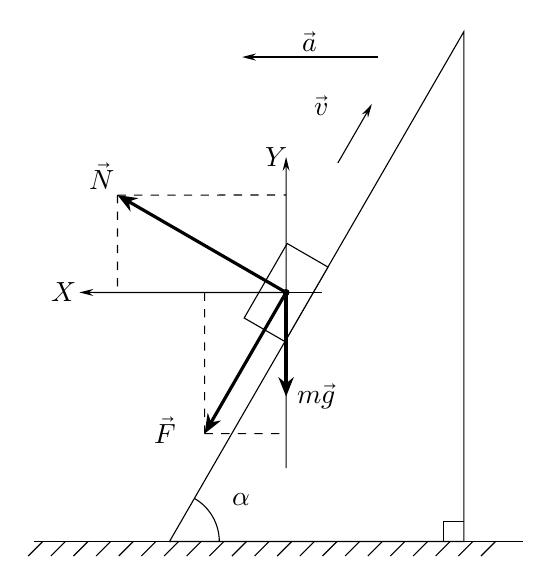
\begin{tikzpicture}[scale=1.15, every node/.style={inner sep=1.5pt}]
        \def\ang{60}
        \def\Ln{2.15}
        \def\Lf{1.8}
        \def\Lmg{1.15}
        % Поверхность, с которой связана система отсчёта
        \foreach \x in {-0.95,-0.70,...,4.25}
            \draw (\x,0) -- ++(-0.16,-0.16);
        \coordinate (A) at (0.45,0);
        \coordinate (B) at (3.7,0);
        \coordinate (C) at (3.7,{3.25*tan(\ang)});
        \fill[white] (A) -- (B) -- (C) -- cycle;
        \draw (A) -- (B) -- (C) -- cycle;
        \draw (-1.05,0) -- (4.35,0);
        \draw ($(B)+(-0.22,0)$) -- ++(0,0.22) -- ++(0.22,0);
        \draw ($(A)+(0.55,0)$) arc[start angle=0, end angle=\ang, radius=0.55];
        \node at ($(A)+({0.92*cos(30)},{0.92*sin(30)})$) {$\alpha$};
        % Груз
        \begin{scope}[shift={(A)}, rotate=\ang]
            \draw[fill=white] (2.55,0) rectangle (3.5,0.52);
            \coordinate (O) at (3.025,0.26);
        \end{scope}
        % Концы сил и их проекции на оси
        \coordinate (Ntip) at ($(O)+({-\Ln*sin(\ang)},{\Ln*cos(\ang)})$);
        \coordinate (Ftip) at ($(O)+({-\Lf*cos(\ang)},{-\Lf*sin(\ang)})$);
        \coordinate (Nx) at (Ntip |- O);
        \coordinate (Ny) at (Ntip -| O);
        \coordinate (Fx) at (Ftip |- O);
        \coordinate (Fy) at (Ftip -| O);
        % Оси: X влево, Y вверх. Тонкие сплошные
        \draw[thin] (O) -- ++(0.4,0);
        \draw[thin, ->] (O) -- ($(Nx)+(-0.42,0)$) node[left] {$X$};
        \draw[thin] (O) -- ($(Fy)+(0,-0.38)$);
        \draw[thin, ->] (O) -- ($(Ny)+(0,0.42)$) node[left] {$Y$};
        % Проекции N и Fтр — тонкий пунктир
        \draw[thin, dashed] (Ntip) -- (Nx);
        \draw[thin, dashed] (Ntip) -- (Ny);
        \draw[thin, dashed] (Ftip) -- (Fx);
        \draw[thin, dashed] (Ftip) -- (Fy);
        % Скорость груза относительно клина — вверх по грани; подпись в стороне от стрелки
        \coordinate (V0) at ($(A)+({4.55*cos(\ang)},{4.55*sin(\ang)})+({-0.48*sin(\ang)},{0.48*cos(\ang)})$);
        \coordinate (V1) at ($(V0)+({0.75*cos(\ang)},{0.75*sin(\ang)})$);
        \draw[->] (V0) -- (V1);
        \node[anchor=south east, inner sep=1pt] at ($(V0)!0.55!(V1)+({-0.1*sin(\ang)},{0.1*cos(\ang)})$) {$\vec{v}_{\text{отн}}$};
        % Силы — толстые
        \draw[line width=1.15pt, -{Stealth[length=7pt, width=5.5pt]}] (O) -- ++(0,-\Lmg) node[right, xshift=2pt] {$m\vec{g}$};
        \draw[line width=1.15pt, -{Stealth[length=7pt, width=5.5pt]}] (O) -- (Ntip) node[above left] {$\vec{N}$};
        \draw[line width=1.15pt, -{Stealth[length=7pt, width=5.5pt]}] (O) -- (Ftip) node[left, xshift=-5pt] {$\vec{F}_{\text{тр}}$};
        \fill (O) circle (1.1pt);
        % Ускорение клина — вдоль оси X
        \draw[->, thick] ($(C)+(-0.95,-0.28)$) -- node[above] {$\vec{a}$} ++(-1.5,0);
    \end{tikzpicture}

    Рис. 1. Силы, действующие на груз, и скорость груза относительно клина (пунктир~— проекции сил на оси)
    \end{center}

    \textbf{Дано:} \(\alpha = 60^\circ\), \(\mu = 0{,}12\). Клин движется по гладкой горизонтальной плоскости, груз скользит по его грани вверх равномерно.

    \textbf{Найти:} ускорение клина \(a\).

    \textbf{Решение.}

    Систему отсчёта свяжем с горизонтальной поверхностью, по которой скользит клин: поверхность покоится, поэтому система инерциальна и силы инерции не вводятся. Начало координат~— в центре груза, ось \(X\) направим горизонтально влево (по ускорению клина), ось \(Y\)~— вертикально вверх.

    \textbf{На груз действуют только три силы:} тяжесть \(m\vec{g}\), реакция опоры \(\vec{N}\) и трение \(\vec{F}_{\text{тр}}\). Ускорение клина само по себе силой не является, поэтому второй закон Ньютона записывается сразу суммой этих трёх сил:
    \[
        m\vec{g} + \vec{N} + \vec{F}_{\text{тр}} = m\vec{a}.
    \]

    \(m\vec{g}\) направлена вертикально вниз. \(\vec{N}\) перпендикулярна грани и отклонена от оси \(Y\) влево на угол \(\alpha\). Груз скользит вверх по грани, поэтому сила трения~— сила трения скольжения,
    \[
        F_{\text{тр}} = \mu N,
    \]
    и направлена вниз по грани, против \(\vec{v}_{\text{отн}}\).

    Клин движется поступательно с ускорением \(a\) вдоль оси \(X\). Относительно клина груз движется равномерно, относительное ускорение равно нулю, поэтому ускорение груза относительно поверхности совпадает с ускорением клина:
    \[
        a_X = a, \qquad a_Y = 0.
    \]

    Проекции трёх сил. На ось \(X\) и реакция, и трение дают составляющие влево; на ось \(Y\) реакция направлена вверх, трение и тяжесть~— вниз:
    \[
        \left\{
        \begin{aligned}
            N\sin\alpha + \mu N\cos\alpha &= ma,\\
            N\cos\alpha - \mu N\sin\alpha &= mg.
        \end{aligned}
        \right.
    \]
    Из уравнения для оси \(Y\)
    \[
        N = \frac{mg}{\cos\alpha - \mu\sin\alpha}.
    \]
    Подставляем в уравнение для оси \(X\) и сокращаем \(m \neq 0\):
    \[
        a = g\frac{\sin\alpha + \mu\cos\alpha}{\cos\alpha - \mu\sin\alpha} = g\frac{\tg\alpha + \mu}{1 - \mu\tg\alpha}.
    \]
    При \(\alpha = 60^\circ\) будет \(\tg\alpha = \sqrt{3}\), поэтому
    \[
        a = g\frac{\sqrt{3} + 0{,}12}{1 - 0{,}12\sqrt{3}}.
    \]
    Численно \(\sqrt{3} \approx 1{,}732\), \(0{,}12\sqrt{3} \approx 0{,}208\):
    \[
        a \approx g\frac{1{,}852}{0{,}792} \approx 2{,}34\,g.
    \]
    При \(g = 9{,}8~\frac{\text{м}}{\text{с}^2}\)
    \[
        a \approx 2{,}34 \cdot 9{,}8~\frac{\text{м}}{\text{с}^2} \approx 22{,}9~\frac{\text{м}}{\text{с}^2}.
    \]

    \textbf{Какие законы использованы и почему они применимы.}

    Второй закон Ньютона. Применим, потому что система отсчёта, связанная с плоскостью, инерциальна; груз можно считать материальной точкой~— он движется поступательно, его размеры в условии не заданы.

    Закон трения скольжения \(F_{\text{тр}} = \mu N\). Груз скользит, коэффициент трения задан, а слово «вверх» фиксирует направление скорости и тем самым направление трения.

    Равенство ускорений груза и клина~— следствие теоремы сложения ускорений: относительное ускорение равно нулю из-за равномерности скольжения, переносное~— это ускорение клина.

    Гладкость горизонтальной плоскости означает, что ускорение клина горизонтально: трения клина о плоскость нет. Масса клина не нужна, так как ищется ускорение, а не сила, которая его сообщает.

    \textbf{Ответ:}
    \[
        a = g\frac{\sqrt{3} + 0{,}12}{1 - 0{,}12\sqrt{3}} \approx 2{,}34\,g \approx 22{,}9~\frac{\text{м}}{\text{с}^2};
    \]
    ускорение направлено горизонтально влево, в сторону острого угла клина.
\end{document}
